% MUST BE A SUBSECTION, NOT A SECTION
Ontology grounding means the detailed description of database structure and content by formal ontology mechanisms. This process requires in-depth domain knowledge, insight into the way databases are populated, as well as ontology engineering skills, based on the understanding of upper level ontology principles and description logics.
Aware that a straightforward,  automatized ``ontologization'' of a database schema is not sufficient, the ontology engineer has to critically assess the pros and cons of competing modelling strategies, in a way that correctly accounts for the underlying domain segment, and which provides enough expressiveness to address typical queries (Fig. \ref{fig:process}). 

This grounding process starts with the identification of typical domain-related queries and their definition as Competency Questions (CQs) \citep{Gruninger1994}. Then databases that are needed to answer these CQs are selected, as well as the ontologies that are referred to by these databases. Ontology annotations in databases as well as database structure and content are identified and linked to the ontology entities they denote, which can be TBox or ABox entities. 

Top-level classes and relations of the domain ontologies are mapped to an upper level ontology. During this mapping process, consistency is iteratively checked by a DL reasoner. Repetitive structures are identified in database records according to the ontology organization and described as generalizable ontology design patterns. In this process, the interdependencies and relationships between the referents and/or their types are analysed, based on domain knowledge, and the need for newly defined subclasses is assessed. 

General patterns are applied to the overall databases or to database subsets under consideration and are formatively evaluated by test queries that were formulated beforehand. When the content generated is logically consistent and the answers to the test queries are complete, the process reaches the end, and the output corresponds to an ontologized interpretation of the database. Otherwise, more iterations and evaluations are required in order to meet consistency, domain validity and user expectations. 
  
\begin{figure}[h]
\centering
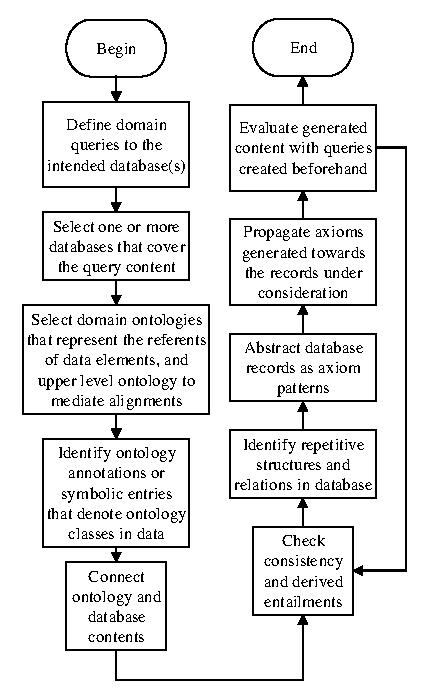
\includegraphics{./PIC/process}
\caption{Ontology grounding process.}
\label{fig:process}
\end{figure}

For assessment and demonstration of the ontology grounding approach we have formulated the following CQs on Hcy metabolism. They explore database content concerning phenotypes, proteins, molecules and biological processes from several organisms, using ontologies and databases described in Section \ref{sec:resources}).

\begin{enumerate}
	\item Which kinds of biological processes related to Hcy can be found in mice?
	\item Which are the proteins that exhibit  \textit{methyltransferase activity}? 
	\item Which are the kinds of biological processes in which proteins of the type \textit{cystathionine gama lyase} participate, exhibiting \textit{carbon-sulfur lyase activity}?
	\item Which dysfunctional biological processes entail a risk of \textit{Myocardial infarction}?
	\item Which kinds of organisms are capable of performing `\textit{cysteine biosynthetic process}'?
	\item Which proteins found in ruminants have the capability of methionine biosynthesis? 
\end{enumerate}

